\chapter{Implementation and Evaluation}
\label{Chapter4}

This chapter describes the product that the design in Chapter~\ref{Chapter3} became, how it was implemented, the cloud deployment used to run and evaluate it, the distribution of the mobile client, the security-hardening process applied to the platform, and an evaluation of the resulting system. It opens from the user's side, walking the journeys the delivered application actually supports, before turning to the engineering that makes them work.

\section{The Product: End-to-End User Journeys}
\label{sec:product}

Chapters~\ref{Chapter1} to~\ref{Chapter3} argue a problem and specify a design. This section shows what was built, from the position of the person it was built for. The five journeys below are not a feature inventory; they are the paths our trial users actually take, in the order a teenager meets them: the ordinary day first, the hard moment second, and professional care only when the first two are not enough. Each is presented as the sequence of screens a user passes through, and each is annotated with the requirements from Section~\ref{sec:requirements} that it exercises, so that the visual walkthrough and the specification can be read against each other.

Two properties are worth stating before the journeys, because they are what makes the sequences below a single product rather than five separate tools. First, every journey reads from or writes to the same record: the daily entries a user makes in the first journey are what the AI companion, the therapist, and a trusted friend later respond to. Second, no journey crosses a data boundary without the user's explicit act. The consent step is not an afterthought bolted onto the professional journey; it is a screen the user visits deliberately, and the last journey is devoted to it.

\subsection{The daily loop: notice, record, understand}
\label{sec:journey-daily}

\begin{figure}[htbp]
    \centering
    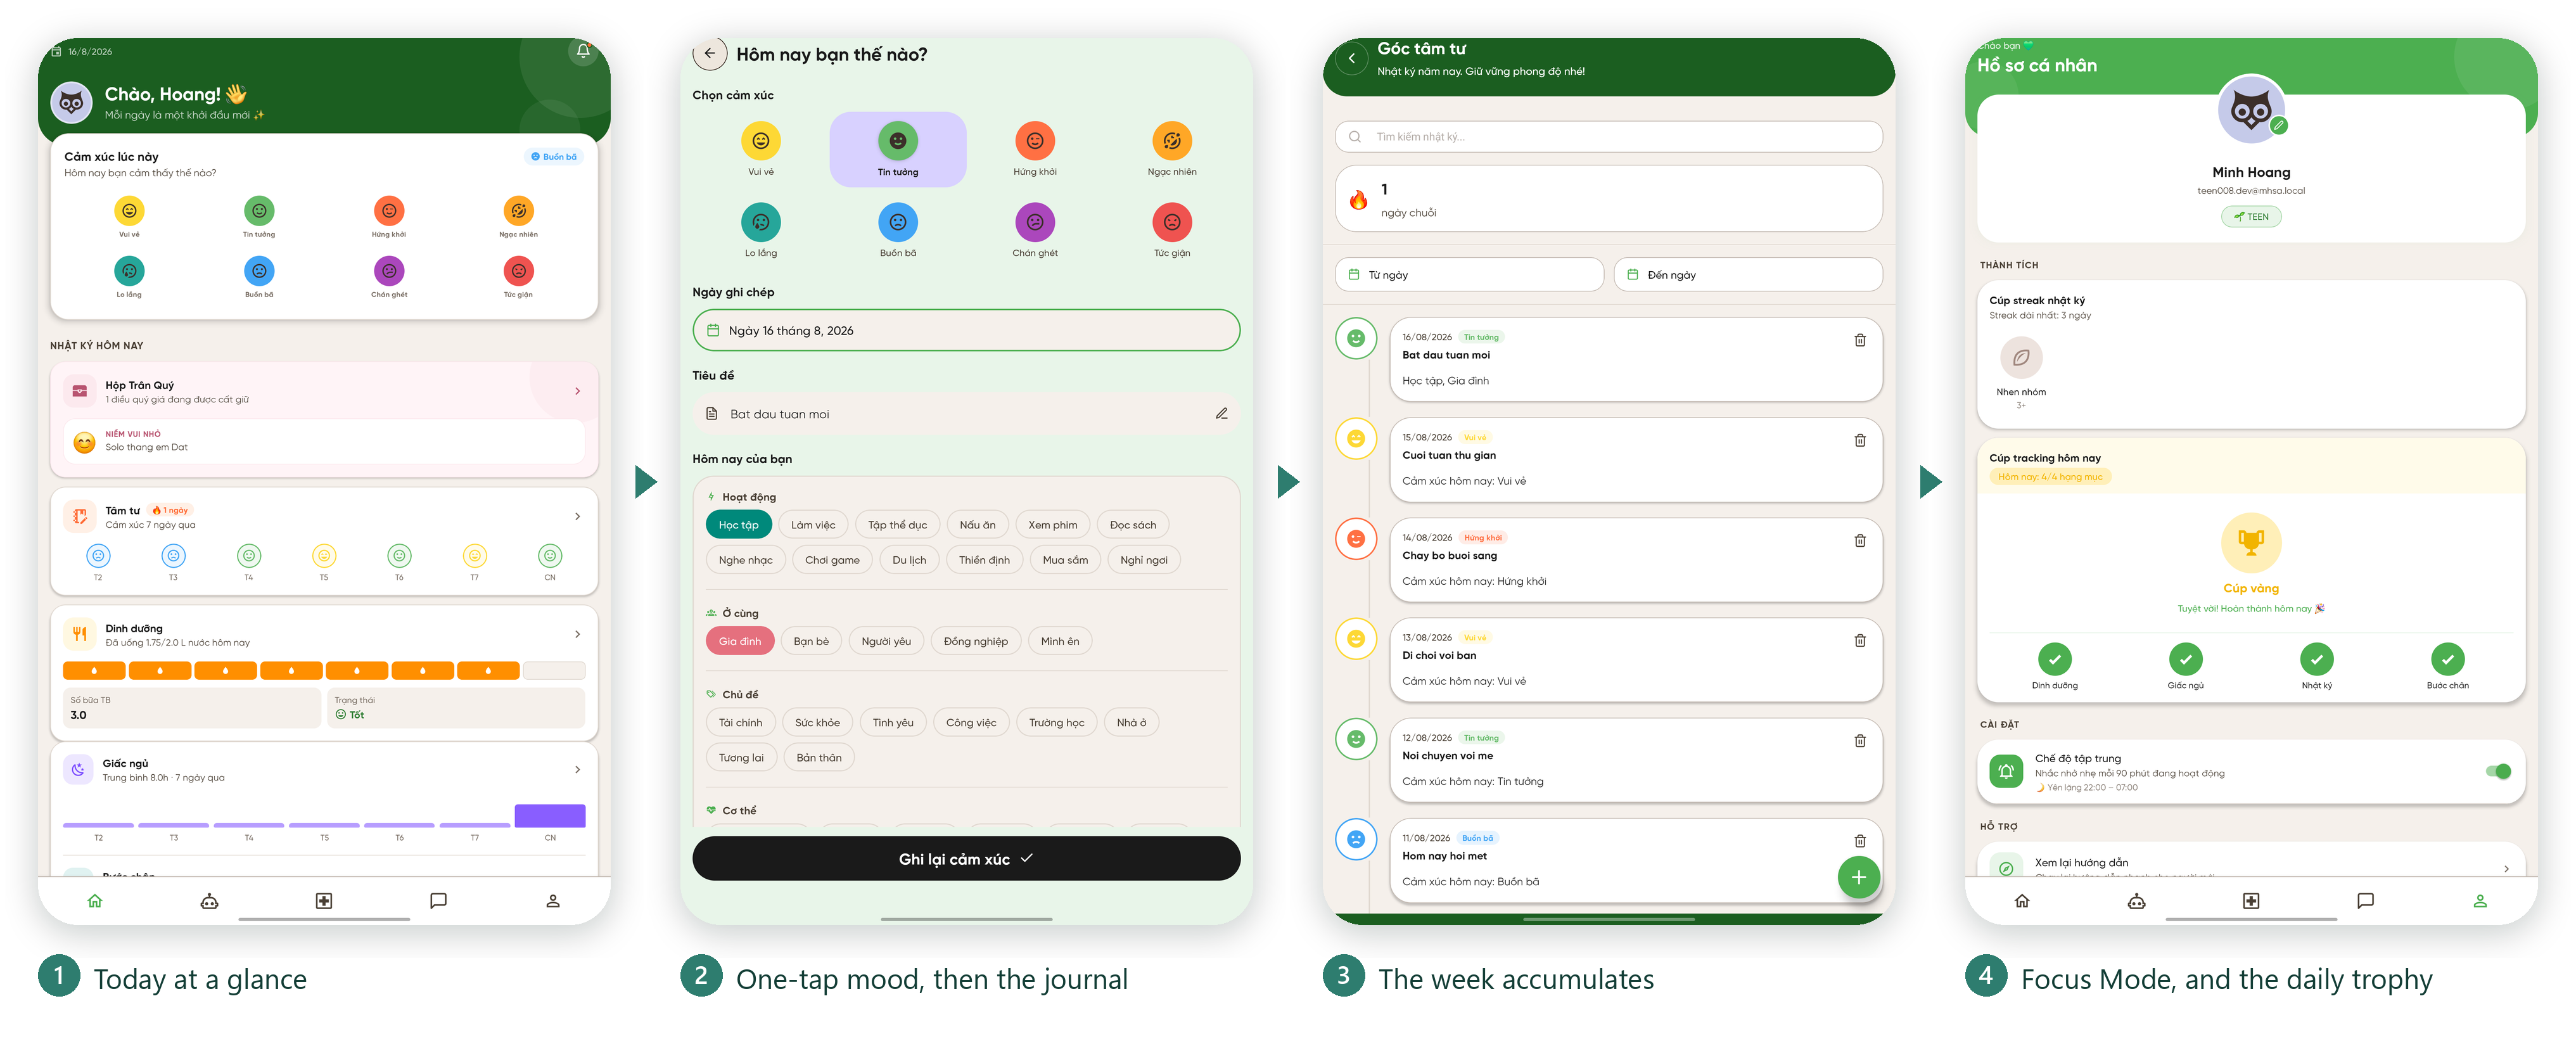
\includegraphics[width=\textwidth]{Chapter4/images/j1-daily-loop.png}
    \caption{The daily loop: a Focus Mode prompt, the mood check-in, the emotional journal, and the trends the entries accumulate into.}
    \label{fig:j1-daily-loop}
\end{figure}

The habit at the centre of the product is a check-in that costs one tap. Figure~\ref{fig:j1-daily-loop} follows it. The application comes to the user rather than waiting to be opened: with Focus Mode enabled, a prompt arrives roughly every ninety minutes through the waking day and falls silent during Quiet Hours, so the recall problem identified in Section~\ref{sec:requirements} is solved without the application becoming a nag (FR3). Acting on the prompt lands the user directly on the check-in, where a mood is chosen and, optionally, a line of context added.

The journal deepens the same act rather than replacing it. A user picks the emotion that fits, names what the day was about, and writes as much or as little as they want, with photographs attached if they help. What the user gets back for this is the fourth screen: a mood calendar that colours each day, per-category streaks, and weekly trends across sleep, steps, nutrition, and breathing (FR1, FR2). This is the return on the habit and the reason it survives past the first week, since the entries stop being data submitted somewhere and become a picture of the user's own month that only they can assemble.

\subsection{The low moment: first aid that is routed, not generic}
\label{sec:journey-low}

\begin{figure}[htbp]
    \centering
    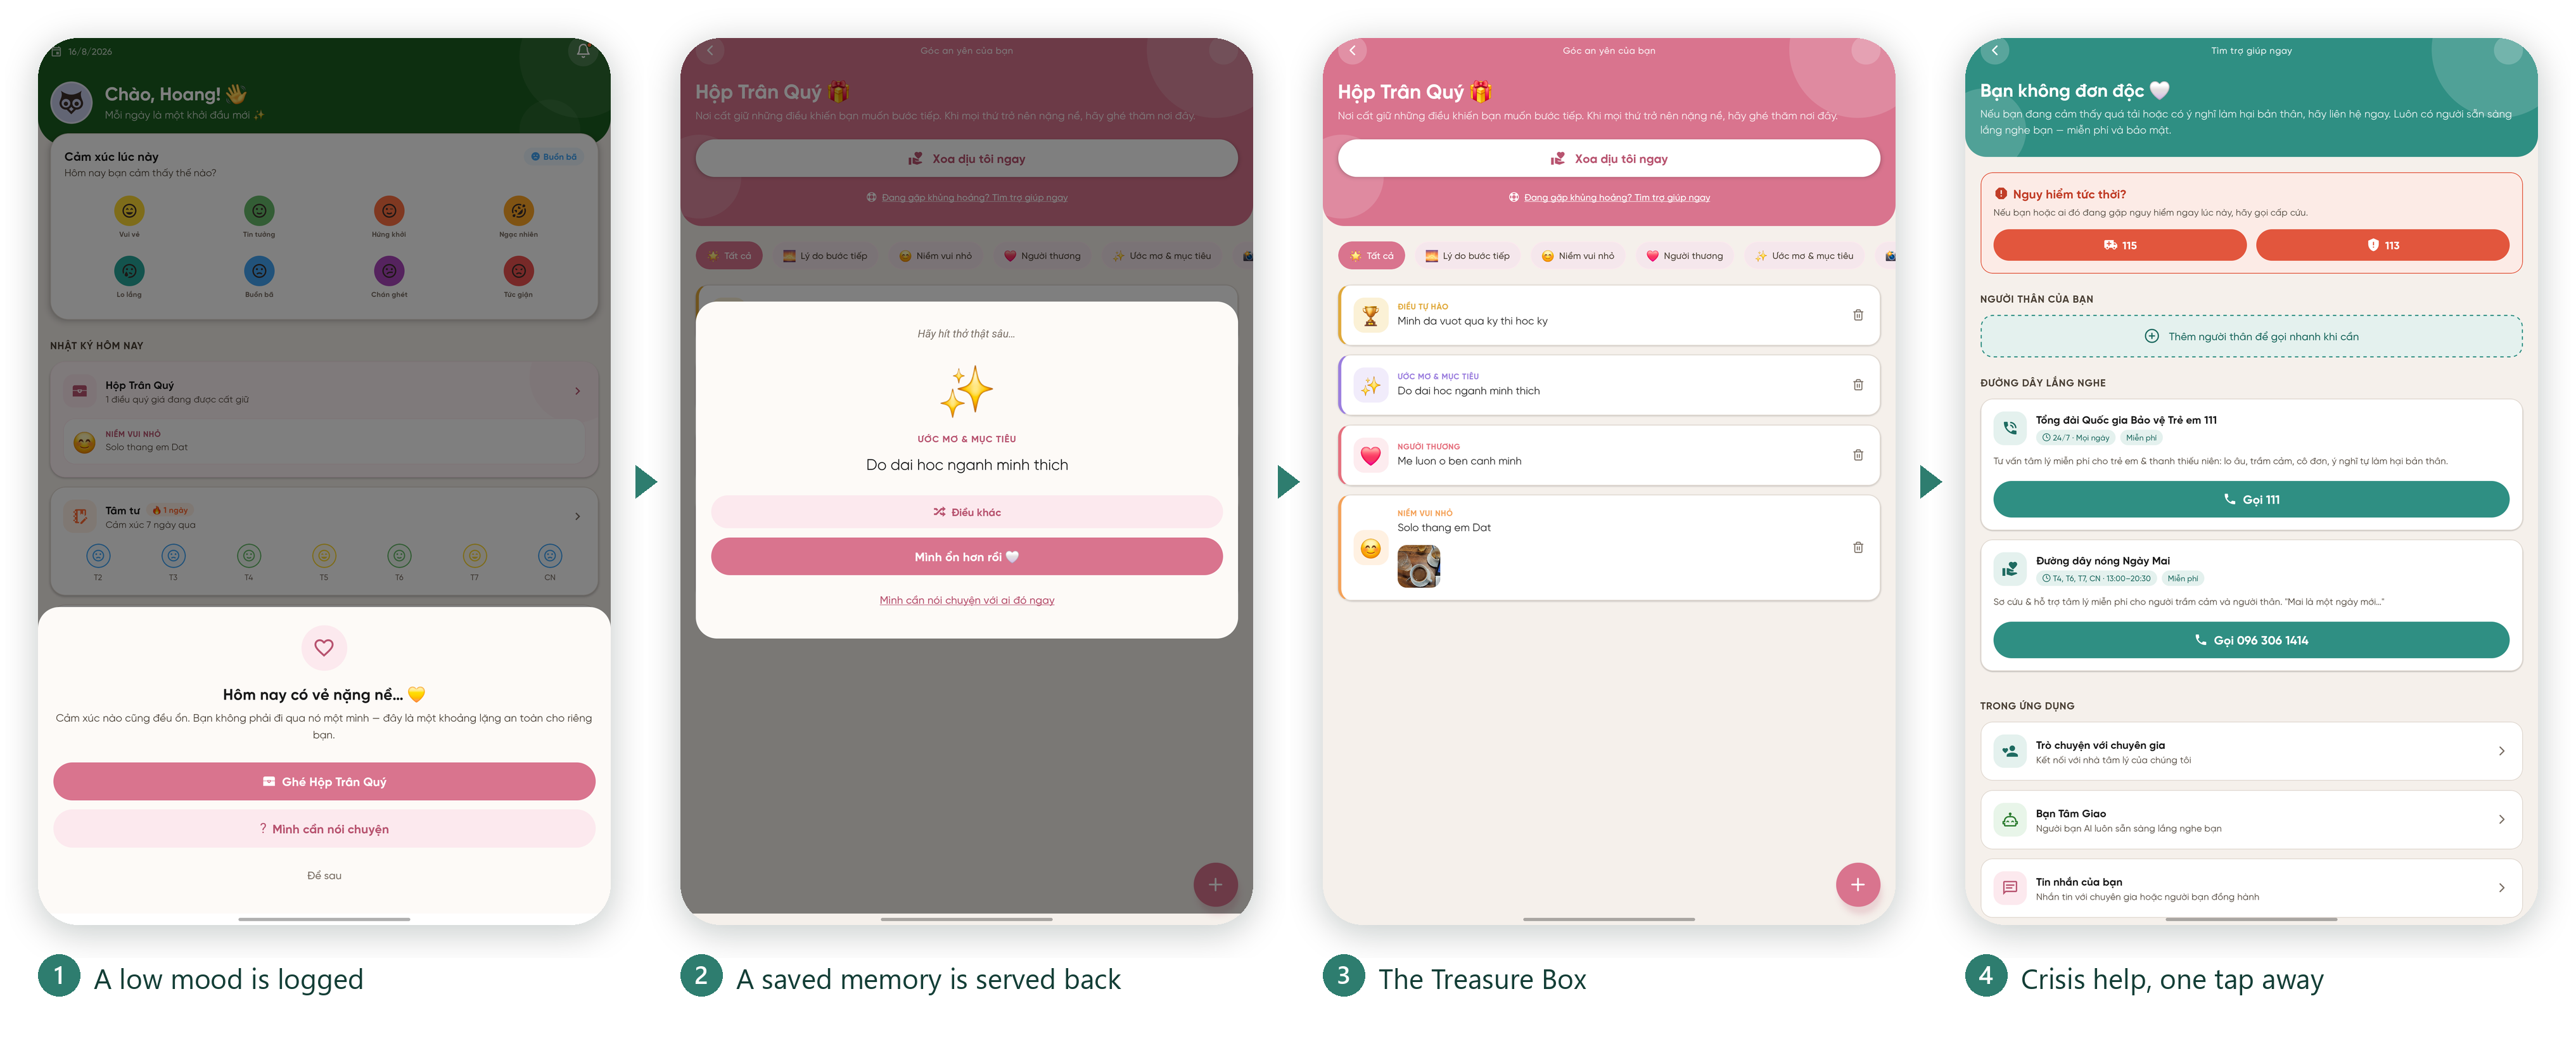
\includegraphics[width=\textwidth]{Chapter4/images/j2-low-moment.png}
    \caption{Logging a negative emotion routes to a matched response: guided breathing for anger, the Treasure Box for sadness, and the emergency area always one tap away.}
    \label{fig:j2-low-moment}
\end{figure}

The design decision that most distinguishes the product is what happens immediately after a negative mood is logged. The application does not return the user to a dashboard. It routes them, and it routes by which emotion was recorded, following the guidance of the professionals consulted in Section~\ref{sec:elicitation}: anger is met with a guided breathing exercise, sadness with the user's own Treasure Box (FR5).

The Treasure Box, shown in the third panel of Figure~\ref{fig:j2-low-moment}, is the feature trial users valued most (Section~\ref{sec:most-valued}). Its premise is that a low mood makes good memories hard to reach, so the memories are saved in advance, on a good day, and reopened on the bad one: photographs, kind messages, small wins, and reasons to keep going, put somewhere the user can find them at the moment recall fails. Running alongside both paths, the emergency area is reachable in one tap from anywhere in the application and renders entirely from client-side content, so it stays available even when the backend is not (FR5).

\subsection{Someone to talk to, at any hour}
\label{sec:journey-companion}

\begin{figure}[htbp]
    \centering
    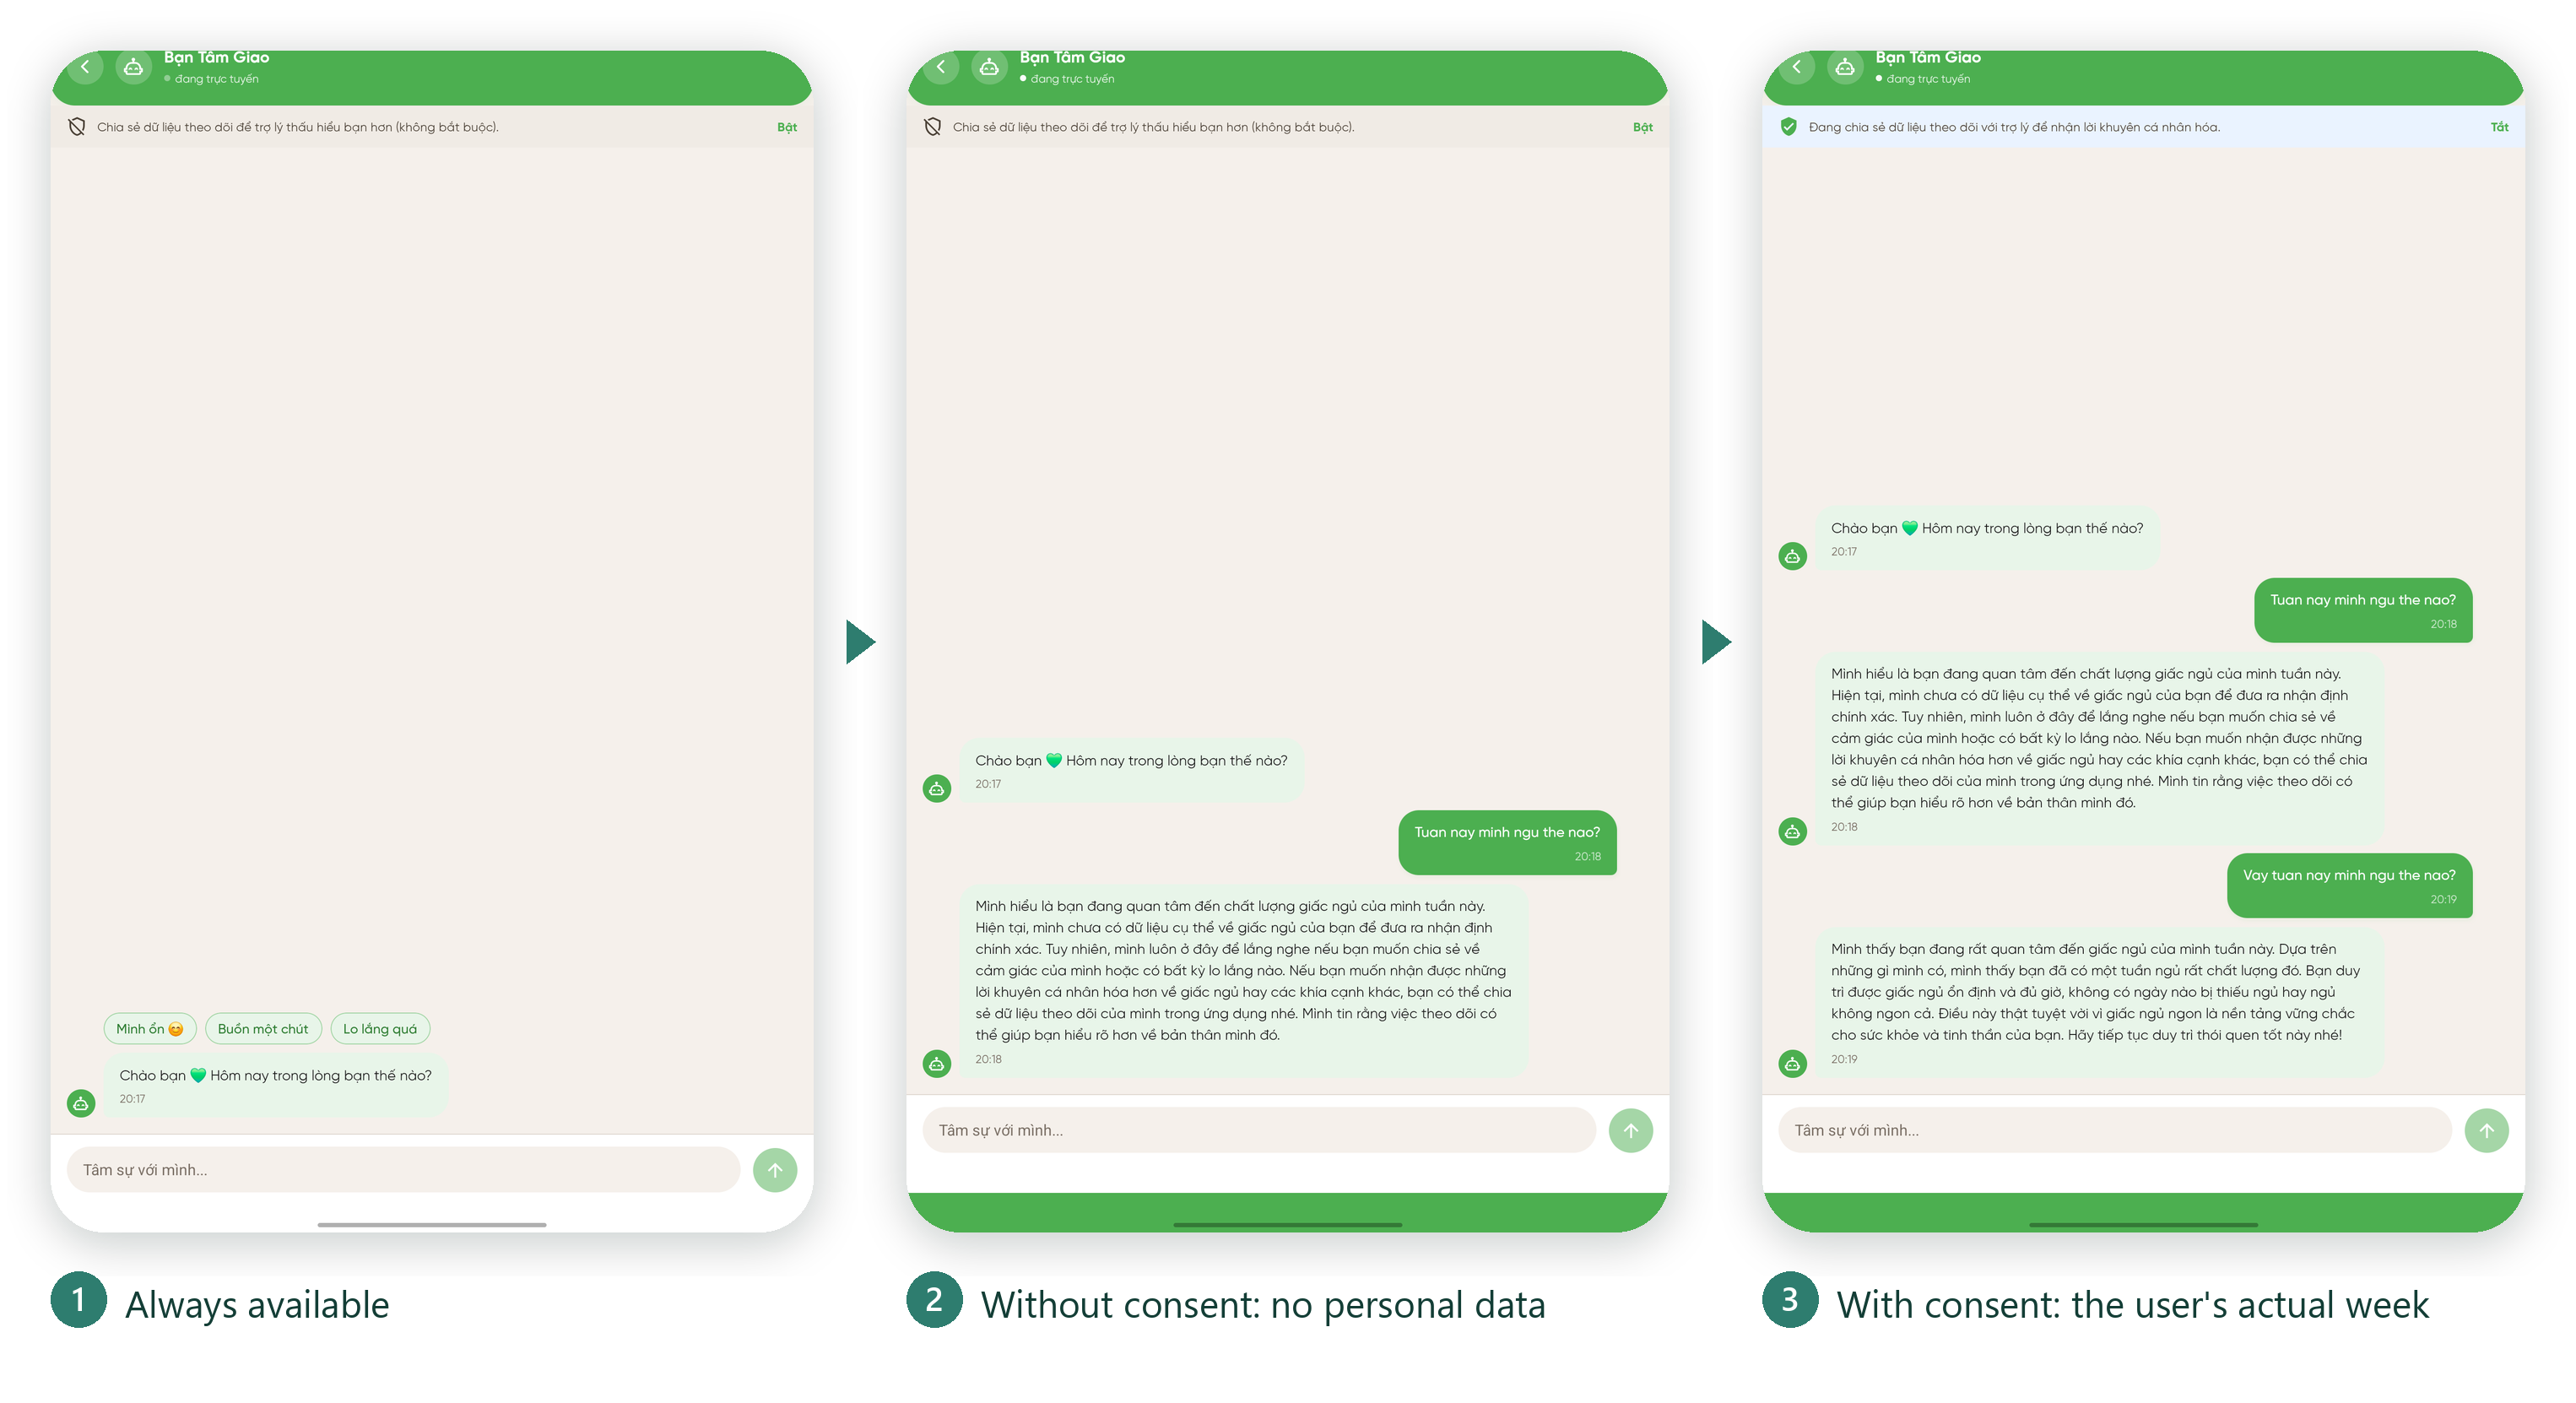
\includegraphics[width=\textwidth]{Chapter4/images/j3-companion.png}
    \caption{B\d{a}n T\^am Giao: an always-available companion whose replies draw on the user's own week when, and only when, access has been granted.}
    \label{fig:j3-companion}
\end{figure}

Trial users reported reaching for the companion late at night, when contacting a friend or a therapist was not an option. That availability is the feature. What separates it from a general-purpose chatbot is that it can be given the user's own recent history, so a reply can respond to a week that actually happened rather than to nothing at all (FR4). The grounding is opt-in and off by default: a user who never grants access still gets a companion, just one without personal context, and the difference between the two is visible in the replies themselves.

The contrast is visible directly in Figure~\ref{fig:j3-companion}: asked the same question twice, the companion first states plainly that it has no sleep data and invites the user to share it, and then, once the grant is switched on in the banner at the top of the conversation, characterizes the week from the user's actual logs. The grounding is nevertheless qualitative rather than numeric, for the reasons set out in Section~\ref{sec:expert-findings}.

The safety behaviour is deliberately narrow. A message matching a small list of self-harm or violence phrases bypasses the model entirely and returns the crisis hotlines directly. This is a within-conversation redirect and not a clinical assessment; the system performs no risk scoring and raises no automated alert to any third party, for the reasons set out in Chapter~\ref{Chapter5}.

\subsection{Crossing into professional care}
\label{sec:journey-professional}

\begin{figure}[htbp]
    \centering
    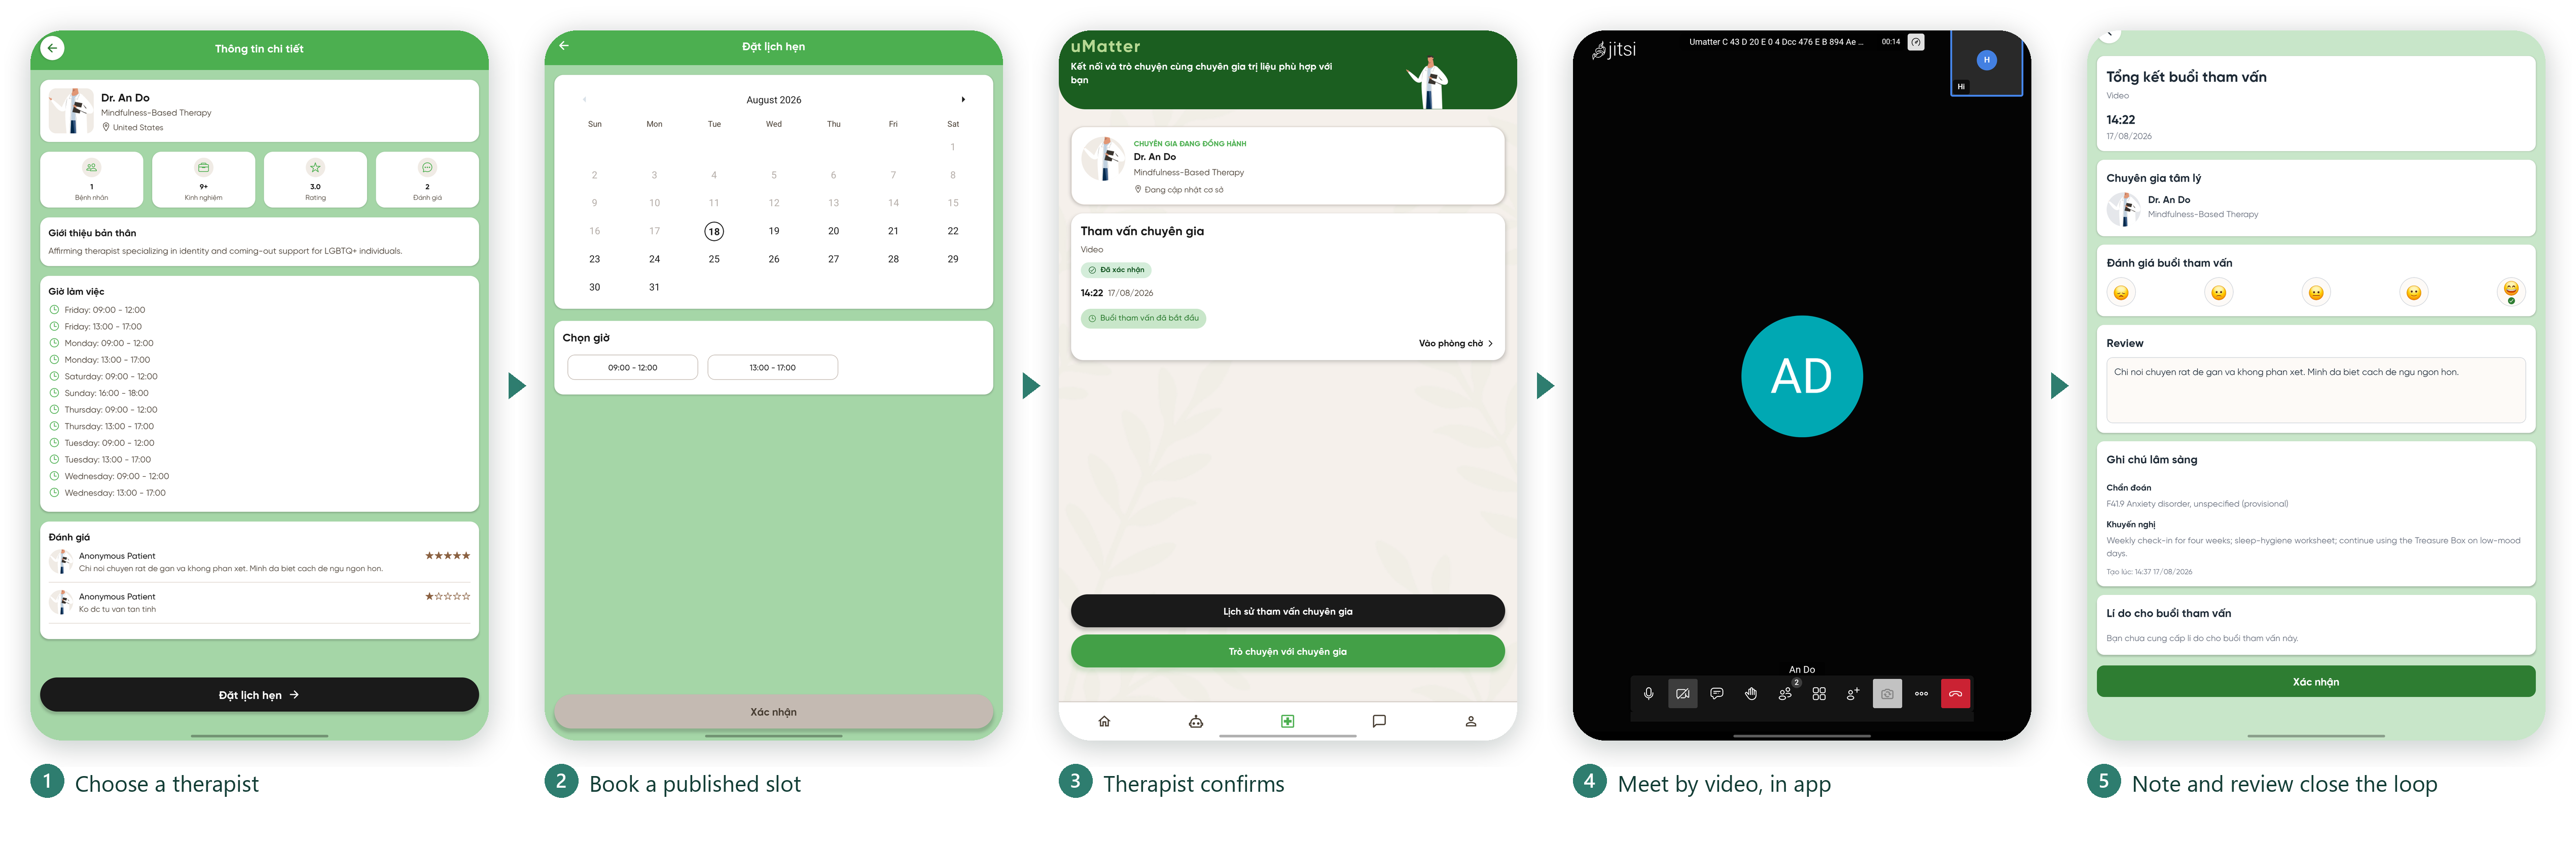
\includegraphics[width=\textwidth]{Chapter4/images/j4-professional.png}
    \caption{From choosing a therapist to sitting in the consultation, without leaving the application.}
    \label{fig:j4-professional}
\end{figure}

When self-help is not enough, the crossing into professional care happens inside the same application. A short intake form asks what the user is going through, how they prefer to be met, and whether prior therapy has been tried, and ranks therapists by the overlap with what each one treats (FR6). Booking is a slot on the therapist's published calendar; confirmation arrives as a push notification and an email so the appointment does not slip past (FR8). The session runs as video inside the application, and afterwards the user reads the therapist's structured note and leaves a review.

Figure~\ref{fig:j4-professional} follows one appointment through that arc. The therapist's profile states what they treat and when they work; the calendar exposes only the slots they have actually published; the appointment then waits, visibly, until the therapist accepts it. The video room opens ten minutes before the hour and no earlier, and the user who arrives first waits in a lobby rather than in an empty room --- the session cannot begin until the therapist is present. The final panel is where the loop closes: the therapist's finalized note, its diagnosis and its recommendations, is presented to the user on the same screen that asks them to rate the session, so reading what the professional concluded and giving feedback on it are a single act rather than two.

The therapist works the other side of the same appointment from the web dashboard described in Section~\ref{sec:professional}. This is the point at which the black box between sessions closes: a therapist who has been granted access opens the consultation already knowing how the patient's month went, instead of spending the first part of the session reconstructing it from memory.

\subsection{Choosing who sees}
\label{sec:journey-consent}

\begin{figure}[htbp]
    \centering
    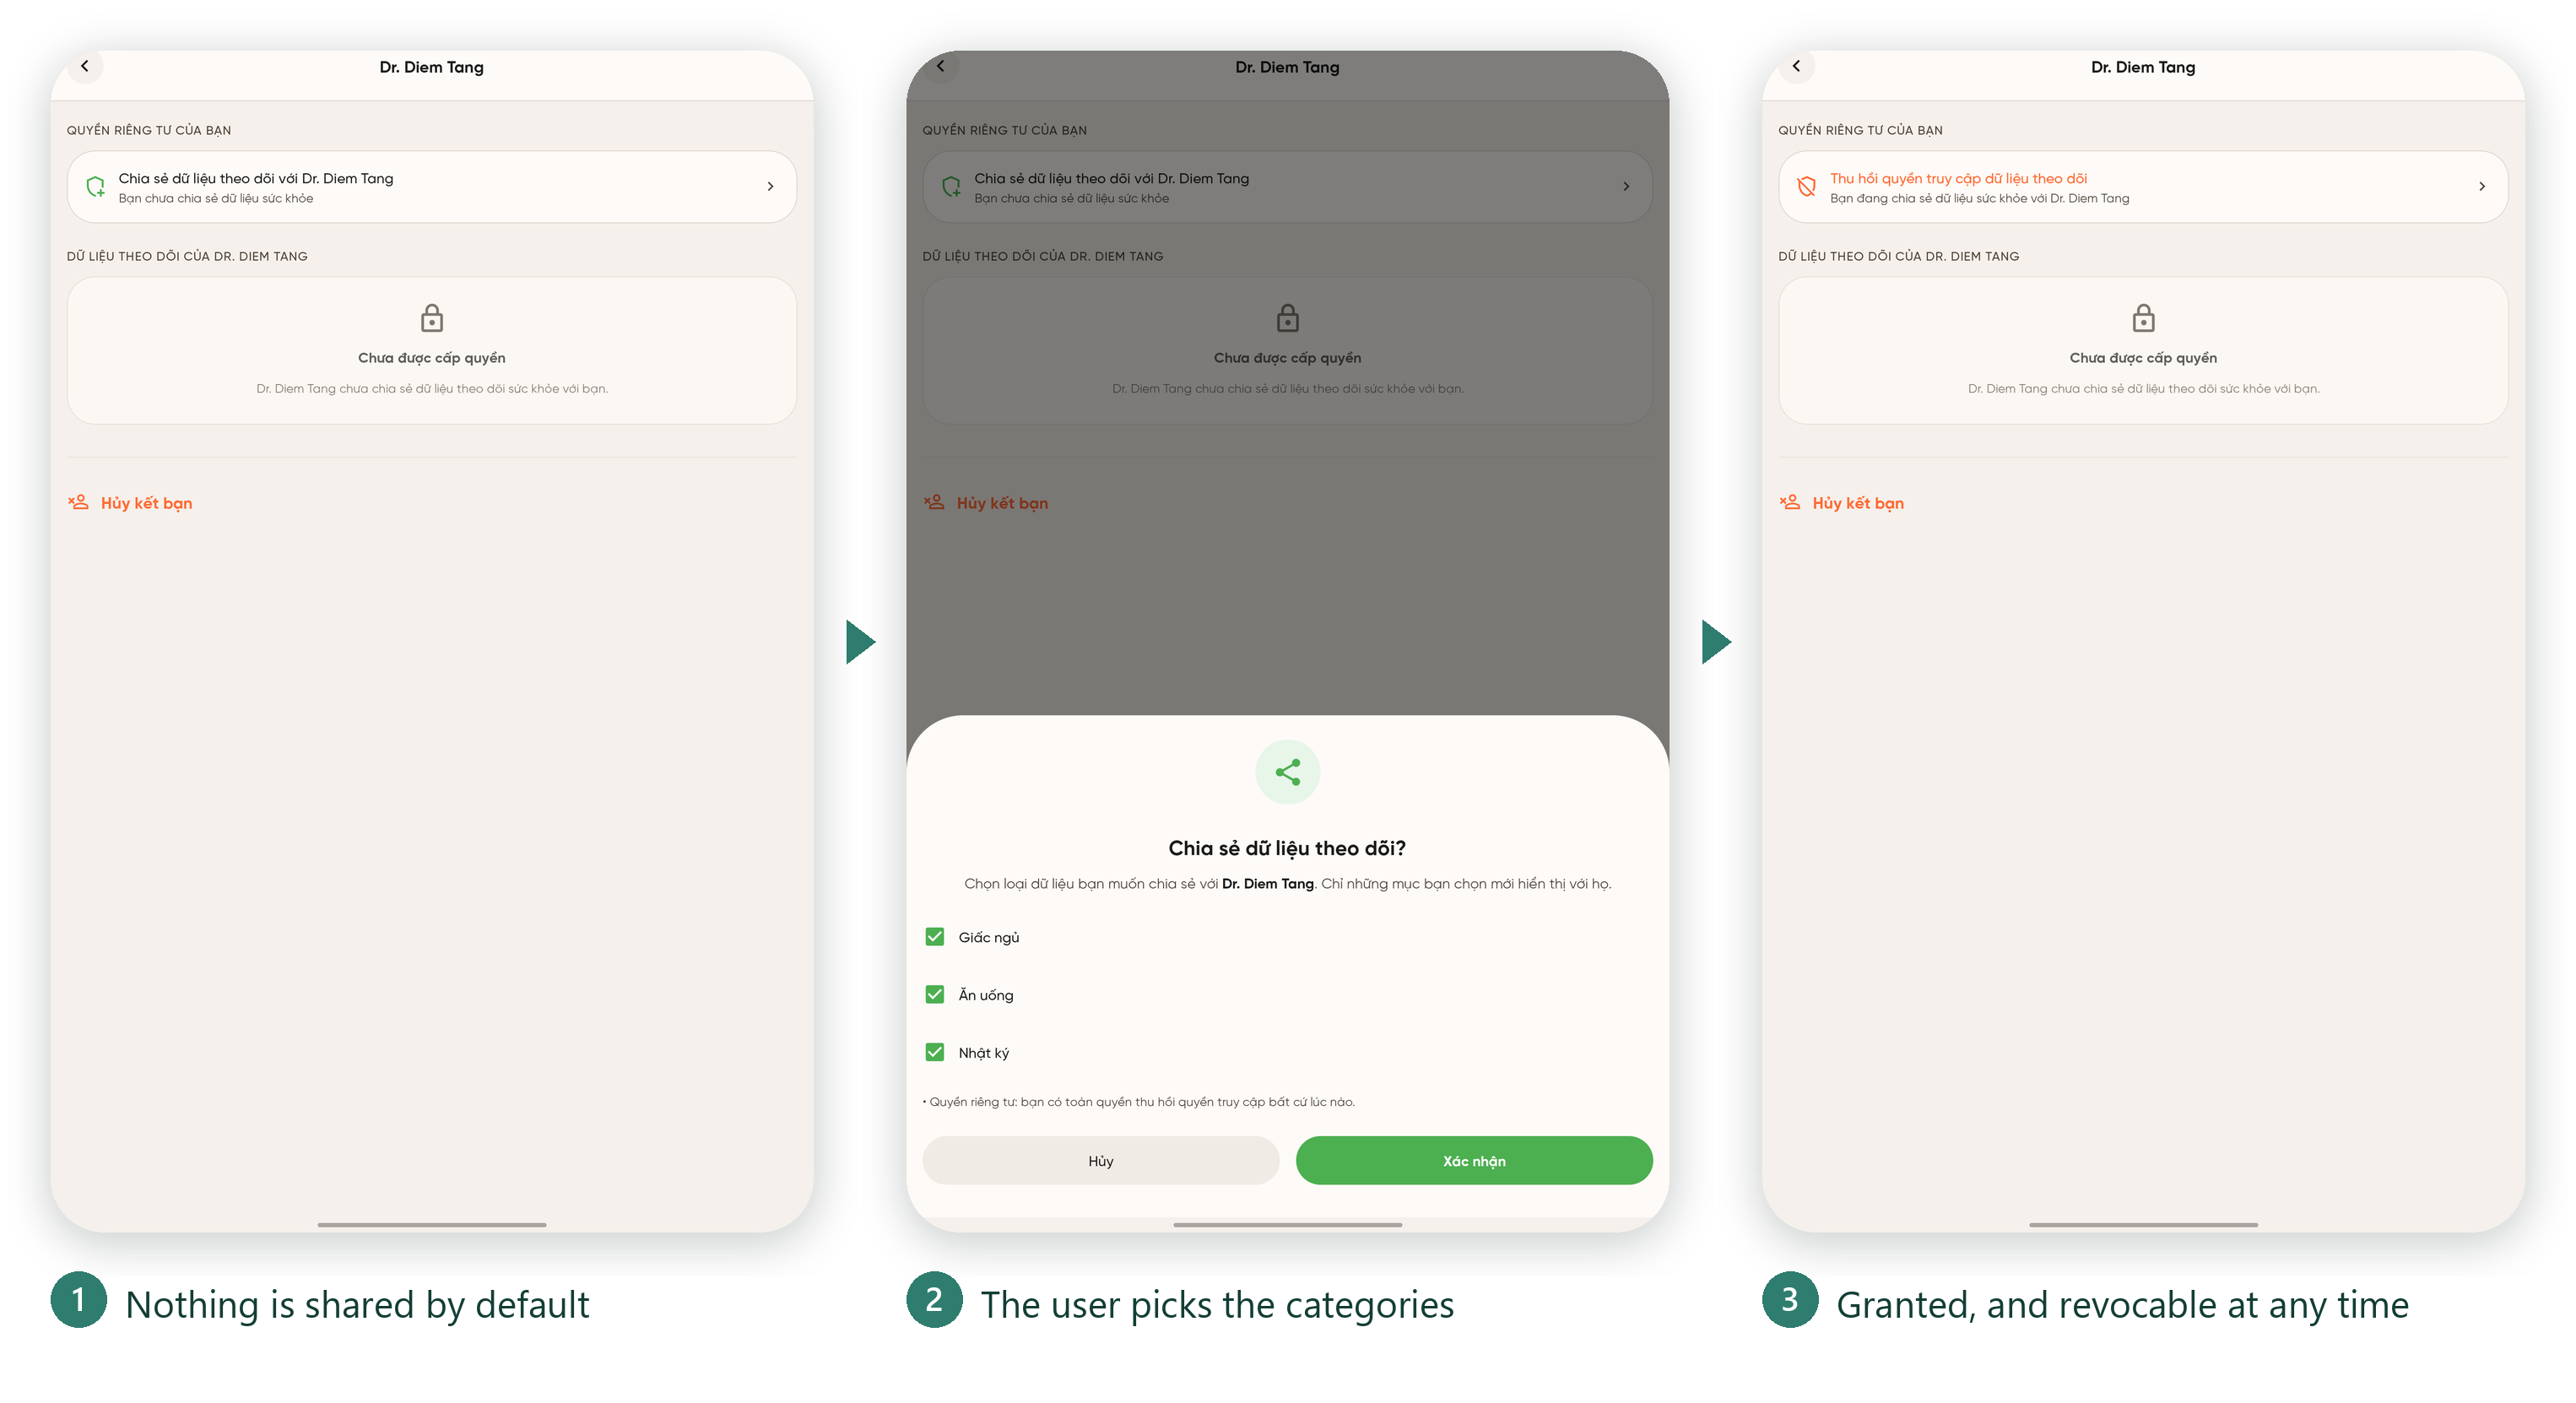
\includegraphics[width=\textwidth]{Chapter4/images/j5-consent.png}
    \caption{One consent mechanism for every audience: nothing is shared until the user selects the categories to expose, and the grant is revocable from the same screen afterwards.}
    \label{fig:j5-consent}
\end{figure}

The final journey is the one that makes the other four safe to use, and trial users identified it as the precondition for writing honestly at all (Section~\ref{sec:expert-findings}). Nothing a user records is visible to anyone by default, and Figure~\ref{fig:j5-consent} follows the grant from that default to an active, revocable share. The screen opens stating plainly that nothing has been shared; the user then chooses which categories of their record to expose, category by category, and confirms. Afterwards the same row inverts into a revoke control, so withdrawing access is exactly as easy as granting it (FR1, FR6, FR7, NFR1). The grant is surfaced wherever the audience appears rather than buried in a settings menu: the banner at the top of the AI conversation in Figure~\ref{fig:j3-companion} is the companion's own grant control, carrying the same meaning and the same server-side enforcement as the grant a user extends to a therapist or a friend.

The point is that this screen is the only way in, for every audience. A therapist, a parent, a friend, and the AI companion are grantees of exactly the same mechanism, enforced server-side. There is deliberately no privileged parental path and no automatic alerting: our baseline study found that automatic crisis alerts to family were rejected as pressure to perform a better mood than the one being felt. A parent therefore sees precisely what their child chose to show them, which is the intended outcome rather than a limitation.

\subsection{What the journeys share}

Table~\ref{tab:journeys} maps each journey to the requirements it exercises. Read together, the journeys are one loop rather than five features: the daily record made in the first is what the second routes on, what the third grounds its replies in, what the fourth gives a therapist to work from, and what the fifth governs access to. This is the unification argued for in Chapter~\ref{Chapter1}, expressed as the path a user walks rather than as a component diagram, and it is the reason a single platform was worth building instead of assembling the same capabilities from four separate products.

\begin{table}[htbp]
  \centering
  \caption{User journeys and the requirements they exercise}
  \label{tab:journeys}
  \begin{tabular}{|l|p{7.4cm}|l|}
    \hline
    \textbf{Journey} & \textbf{What the user does} & \textbf{Req.} \\
    \hline
    Daily loop & Responds to a Focus Mode prompt, logs a mood, writes a
                 journal entry, reads back the week. & FR1--FR3 \\
    \hline
    Low moment & Logs a negative emotion and is routed to breathing, the
                 Treasure Box, or the emergency area. & FR5 \\
    \hline
    Companion & Talks to the AI at any hour, optionally grounded in their
                own record. & FR4 \\
    \hline
    Professional & Completes intake, books a slot, attends by video, reads
                   the note, leaves a review. & FR6, FR8 \\
    \hline
    Consent & Grants scoped access to a therapist, parent, friend, or the
              companion, and revokes it. & FR7, NFR1 \\
    \hline
  \end{tabular}
\end{table}

\section{Implementation Overview}

The backend services are implemented in Java 17. The Auth, Tracking, AI, and Dashboard services are built on Spring Boot~4.0 and organized as a Maven multi-module project so that shared code (for example, JWT validation logic) is written once and reused. The Therapist service is a separate Gradle project on Spring Boot~4.0, while the Social and Notification services are Gradle projects on the slightly earlier Spring Boot~3.3, reflecting when they were added to the system. Persistence throughout uses Spring Data JPA over PostgreSQL. The Social service's real-time chat is implemented with STOMP over WebSocket, and the Notification service integrates Firebase Cloud Messaging for push delivery in addition to email and an in-app inbox.

On the client side, the mobile application for teenagers is built with React Native~0.83 and React~19 in TypeScript, and the therapist-facing web dashboard is built with React~18, TypeScript, Vite, and Tailwind CSS. Appendix~\ref{Appendix5} records why these platforms, the database, and the language model behind the AI companion were preferred to the alternatives considered.

\section{Deployment}

uMatter was originally deployed on Oracle Cloud Infrastructure (OCI). During the course of this thesis, the deployment was migrated in full to Microsoft Azure, under an Azure for Students subscription. The migration involved:

\begin{itemize}
\item Resolving Azure region-policy restrictions that initially blocked the target subscription from provisioning a virtual machine in the desired region.
\item Configuring Network Security Group (NSG) rules to open the ports required by the API gateway and by directly-exposed services (for example, RabbitMQ's management port during setup, and ports 80 and 443 for the reverse proxy).
\item Working around Azure Cloud Shell setup issues encountered while preparing the target VM.
\item Reproducing the auto-shutdown behavior available on the previous provider using Azure's built-in scheduled auto-shutdown, to control cost under the student subscription, with the containers configured to restart automatically on boot so they come back up automatically when the VM is next started.
\end{itemize}

The resulting deployment runs on a single, right-sized Azure VM hosting 20 containers: multiple Spring Boot JVM services, several PostgreSQL instances (one per owning service), RabbitMQ, Redis, MinIO, and pgAdmin. HTTPS routing is provided by Caddy as a reverse proxy, with DuckDNS supplying a stable hostname for the VM's dynamic address, and the VM's public IP configured as static so the hostname does not need to be re-pointed after the nightly auto-shutdown cycle. This mirrors the general topology described in Chapter~\ref{Chapter3}, with Caddy taking the reverse-proxy/HTTPS-termination role and Nginx continuing to serve as the internal API gateway between the proxy and the backend services.

\subsection{Mobile Application Distribution}

The mobile client for teenagers/patients was packaged and published to the Google Play Store, rather than distributed as a manually installed APK. Publishing through Google Play means end users install and update the app the same way as any other Android application, without needing to trust or manually side-load a build shared outside the store.

This distribution choice also shaped a concrete backend requirement: the published app communicates with the API gateway exclusively over HTTPS on port 443, because modern Android builds block plaintext HTTP traffic by default. Terminating TLS correctly at the reverse proxy, using a Let's Encrypt certificate obtained over port 80, was therefore not an optional hardening step but a hard prerequisite for the Play Store build to reach the backend at all. This is why ports 80 and 443 were treated as non-negotiable when the NSG rules were configured.

\section{Security Hardening}

Because uMatter handles sensitive personal data and coordinates real appointments, the implemented services were subjected to structured security audits organized around the OWASP Top~10 risk categories~\cite{2021-OWASP-Top10}, covering three areas in particular:

\begin{itemize}
\item \textbf{Business logic correctness}: verifying that workflows such as matching, booking, and permission granting behave correctly under normal and adversarial input, not only in the happy path.
\item \textbf{Access control}: specifically JPQL injection patterns in hand-written queries, insecure direct object references (for example, a user supplying another user's record identifier to an endpoint that does not re-check ownership), and mass assignment (a client supplying extra fields in a request body that get bound to fields the client should not be able to set, such as a role or a permission flag).
\item \textbf{Data integrity}: ensuring that concurrent requests cannot leave the system in an inconsistent state.
\end{itemize}

The most significant data-integrity issue identified was a race condition in appointment booking: two concurrent requests to book the same therapist for the same time slot could both pass an application-level availability check before either write was committed, resulting in a double booking. This was closed not by adding an application-level lock, which would not be safe against multiple service instances, but by making the slot claim a single atomic database operation: booking a slot is a conditional update that sets the slot's booked flag to true only where it is still false, so exactly one of two concurrent requests updates a row and the other is rejected. A unique constraint on the appointment's slot reference backs this up as a second line of defense. Because the guarantee lives in the database itself, it holds regardless of how many instances of the Therapist service are running concurrently.

The most significant access-control finding was in the AI service's own path to a user's tracking data, rather than in a caller manipulating another user's identifier. The Tracking service's internal context endpoint, used by the AI service to retrieve grounding data, was reachable by any authenticated internal caller. It performed no check that the caller had actually been granted access to that data, relying instead on network-level trust between services. This is precisely the class of implicit trust that the permission-based data-sharing model in Section~\ref{sec:datasec} is designed to remove. The fix followed the same pattern used elsewhere in the codebase: the AI companion was added as a reserved grantee in the existing access-grant table, and the context endpoint now checks for an active grant before returning anything, exactly as it already did for a therapist. No new authorization mechanism was introduced; an existing one was extended to a caller that had previously been exempted from it.

\section{Evaluation}

The system was evaluated along several dimensions: functional completeness against the design goals in Chapter~\ref{Chapter1}, security posture after hardening, feature positioning relative to the competitive landscape reviewed in Chapter~\ref{Chapter2}, and qualitative feedback from trial users and mental-health professionals, including the features they valued most and the wider findings that emerged from the design, trial, and consultation process.

\subsection{Functional Completeness}
\label{sec:functional-completeness}

All seven backend services described in Chapter~\ref{Chapter3} are implemented and deployed, and both client applications (mobile for teens, web for therapists) are functional against them. Table~\ref{tab:traceability} in Appendix~\ref{Appendix3} traces each requirement from Section~\ref{sec:requirements} to its implementation status.

Every requirement is met except FR8: all three notification channels (push, email, and the in-app inbox) work and fire end-to-end for appointment booking, but the other domain events intended to raise notifications are not currently wired to producers, so coverage across events is partial.

\subsection{Security Posture}

The structured audits identified and closed concrete issues in each of the three areas examined (business logic, access control, and data integrity), including the appointment-booking race condition described above. This does not constitute a formal, independent penetration test, and should be read as an internal hardening pass rather than a certification of the system's security; further external review would be a reasonable next step before any production use involving real users.

\subsection{Comparison with Existing Platforms}

Revisiting the comparison in Table~\ref{tab:competitive}, the implemented system delivers on the feature combination that motivated this thesis: self-care tracking, an AI companion grounded in the user's own data, and peer social features, alongside licensed-therapist matching, booking, video consultation, and clinical notes, connected by a permission-based sharing model that none of the compared single-purpose platforms offer in combination. The clearest gap relative to mature commercial platforms such as BetterHelp and Talkspace~\cite{BetterHelp,Talkspace} is operational maturity: those platforms have been hardened and scaled in production for years, whereas uMatter, as a thesis project, has been validated on a single-VM deployment and an internal security-audit process rather than at production scale.

\subsection{Most-Valued Features}
\label{sec:most-valued}

\subsubsection{The Treasure Box (Hộp Trân Quý)}

The Treasure Box is a personal store of positive ``core memories'' (photos, kind messages, small wins, life goals, and motivating reflections) that a user saves ahead of time and reopens whenever they need comforting. On a low day, when negative bias makes good memories hard to recall, this pre-saved anchor gives users self-compassion they can reach for exactly when they need it. The feature grew directly out of expert collaboration: Miss Pham Thi Thanh Qui first suggested reconnecting users with their reasons for living when feeling low, and mister Vuong Nguyen Toan Thien, CEO of LUMOS, concretized that idea into the Treasure Box, grounding it in research on positive memory and mood. Within the app it is one destination in uMatter's ``psychology first-aid'' response to a low mood, alongside guided breathing and the SOS crisis contacts.

\subsubsection{Daily Reflective Tracking}

Daily reflective tracking is the everyday self-check-in habit at the heart of the app: mood check-ins, the emotional journal, logs for sleep, nutrition, and water, automatic step counting, and guided breathing, each surfaced as a friendly ``today'' card with weekly trends. Doctor Pham Tran Thanh Nghiep assessed these features as ``already very good'' and helpful to users' mental wellbeing, and Miss Qui, holding that physical and mental health are inseparable, endorsed the physical-health tracking (steps, sleep, nutrition, breathing) as a legitimate mental-health signal. Gentle Focus-Mode reminders roughly every ninety minutes, daily achievement ``trophies'' for a completed chain of self-care tasks, and streaks keep it a low-friction habit rather than a chore. The same daily data also grounds the AI companion, the therapist's view (under permission), and the trusted-friend view, so the feature most valued on its own is also what makes the rest of the platform work.

\subsection{Key Findings}
\label{sec:expert-findings}

\subsubsection{Findings from the Design and Development Process}

% TODO: viết lại. Ý chính (rút ra từ Chapter 3 & 4):
\begin{itemize}
\item \textbf{A weekly review cycle kept the feature set close to what users actually asked for.} Development was never carried out in isolation from the people it was for: each phase closed with a meeting held either with the mental-health professionals or with the trial users, and with weekly supervision from the advisor, so a proposed function was argued for, built, and then judged by someone outside the team within the same phase (Section~\ref{sec:elicitation}, Appendix~\ref{Appendix6}). The cost is visible as features removed rather than added, which is the point: the surveys below were dropped, and the Treasure Box was added, because the review said so rather than because the team preferred it.

\item \textbf{Unifying self-care and therapy is feasible behind one permission model.} A single microservices platform can serve both halves of the care journey without merging the data, as long as sharing is explicit, granular, and revocable.
\item \textbf{Network-level trust between services is not enough.} The most instructive security finding was that an internal caller (the AI service) could reach a user's tracking data with no explicit grant, meaning that implicit inter-service trust is exactly the class of assumption the permission model must remove, even for internal callers.
\item \textbf{Grounding the AI in the user's own data}, with a safe fallback, is what makes it useful without over-reaching. Toggling the grant changes the companion's replies materially: without it the AI states plainly that it has no tracking data, while with it the same question draws a reply reflecting the user's actual sleep, mood, and nutrition patterns. The grounding is nevertheless \emph{qualitative}. The companion characterizes the week (``your sleep has not been deep or long enough'') but never quotes a figure, even when explicitly asked for one. Two deliberate choices produce this: the system prompt forbids reciting the context mechanically, to keep the tone conversational rather than clinical, and the context passed to the model is itself an aggregate summary (an average, a count of poor nights, a set of mood tags) carrying no per-day values or dates. The companion is therefore demonstrably personalized but not \emph{verifiable}: a user cannot check a reply against the numbers they logged.
% \item \textbf{[placeholder]} % TODO: thêm finding kỹ thuật khác nếu cần.
\end{itemize}

\subsubsection{Findings from User Feedback}

The findings below come from the seven trial users listed in Appendix~\ref{Appendix6}: they were interviewed for user stories before implementation began and re-interviewed against the working build as each development phase closed, in semi-structured sessions held roughly monthly, alternating with the expert consultations. A separate cohort of seventeen testers exercised the published Android build over the fourteen-day Google Play closed-testing period; that cohort reported defects rather than design opinions, and its output is release-phase testing rather than user research. The trial group is small and drawn from the team's own circle, so what follows is qualitative and carries no statistical weight.

\begin{itemize}
\item \textbf{Daily journaling beats periodic surveys.} Trial users found the weekly/monthly surveys redundant next to the daily journal and 3-hourly mood check-ins; the surveys were dropped.
\item \textbf{The most-loved features were the Treasure Box and daily tracking} (Section~\ref{sec:most-valued}).
\item \textbf{The consent gate is what made honest journaling possible.} Users reported writing honestly in the emotional journal only once they understood that a therapist or a trusted friend sees nothing without an explicit grant that they can revoke at any time. 
\item \textbf{The AI companion was valued for availability, yet the efficiency of the interaction needs improvement.} Users reached for the companion late at night, when contacting a friend or a therapist was not an option. However, the companion's replies is too vague and inefficient and barely reflective of user's actual data even when grounded, making it far inferior to a stronger Gemini or ChatGPT model without a any previous context. 
\end{itemize}

\subsubsection{Findings from Expert Consultations}

\begin{itemize}
\item \textbf{Miss Qui} endorsed the option-based emotional journal, the gentle 3-hourly mood check-ins (for complete, meaningful data and for helping users pay attention to themselves), the 4-7-8 breathing exercise as a response to anger, the reward/trophy loop for completing a chain of self-care tasks, the revocable trusted-person sharing, and physical-health tracking such as steps.
\item \textbf{Mister Thien} praised the Treasure Box concept, the emotion timeline for complete mental-health data, the ``psychology first-aid'' bundle for negative moods (breathing, SOS contact, Treasure Box), and the SOS hotline page.
\item \textbf{Doctor Nghiep} gave the strongest endorsement of the daily reflective tracking features (``already very good'').
\end{itemize}
